\documentclass[10pt]{beamer}
\usepackage{inputenc}
\usepackage{graphicx}
\usepackage{enumerate}
\usepackage{listings}
\usepackage{caption}
\captionsetup{font=scriptsize,labelfont=scriptsize}
\usepackage{amsmath}
\usepackage{amssymb}
\usepackage{amsthm}
\usetheme{metropolis}    
\usepackage{hyperref}
\usepackage{verbatim}
\usepackage{alltt}
\usepackage{xcolor}
\usepackage{appendixnumberbeamer}
\usepackage{subcaption}
\usepackage{animate}
\usepackage{xmpmulti}
\usepackage{threeparttable, longtable}
\usepackage{booktabs}
\usepackage{setspace}



\def\signed #1{{\leavevmode\unskip\nobreak\hfil\penalty50\hskip1em
		\hbox{}\nobreak\hfill #1%
		\parfillskip=0pt \finalhyphendemerits=0 \endgraf}}

\newsavebox\mybox
\newenvironment{aquote}[1]
{\savebox\mybox{#1}\begin{quote}\openautoquote\hspace*{-.7ex}}
	{\unskip\closeautoquote\vspace*{1mm}\signed{\usebox\mybox}\end{quote}}
\newcommand{\backupbegin}{
	\newcounter{finalframe}
	\setcounter{finalframe}{\value{framenumber}}
}
\newcommand{\backupend}{
	\setcounter{framenumber}{\value{finalframe}}
}
\usepackage[normalem]{ulem}
\useunder{\uline}{\ul}{}
\makeatletter
\setbeamertemplate{footline}
{
	\leavevmode%
	\hbox{%
		\begin{beamercolorbox}[wd=.15\paperwidth,ht=2.25ex,dp=1ex,center]{institute in head/foot}%
			\usebeamerfont{title in head/foot}%
			%  \insertshortauthor 
		\end{beamercolorbox}%
		\begin{beamercolorbox}[wd=.6\paperwidth,ht=2.25ex,dp=1ex,center]{institute in head/foot}%
			\usebeamerfont{title in head/foot}%
			\insertshorttitle
		\end{beamercolorbox}%
		\begin{beamercolorbox}[wd=.15\paperwidth,ht=2.25ex,dp=1ex,center]{institute in head/foot}%
			\usebeamerfont{title in head/foot}%
			\insertshortdate
		\end{beamercolorbox}%
		\begin{beamercolorbox}[wd=.1\paperwidth,ht=2.25ex,dp=1ex,right]{institute in head/foot}%
			\usebeamerfont{title in head/foot} 
			\insertframenumber{} / \inserttotalframenumber\hspace*{2ex} 
	\end{beamercolorbox}}%
}

\definecolor{blueucl}{RGB}{0,87,156} 
\setbeamercolor{itemize item}{fg = blueucl}
\setbeamercolor{itemize subitem}{fg = blueucl}
\setbeamercolor{enumerate item}{fg = blueucl}
\setbeamercolor{enumerate subitem}{fg = blueucl}
\setbeamertemplate{itemize item}[triangle]
\setbeamercolor{progress bar}{fg=blueucl}
\setbeamercolor{alerted text}{fg = blueucl}

\lstset{numbers=left, numberstyle=\tiny, stepnumber=1,firstnumber=1,
	numbersep=5pt,
	stringstyle=\ttfamily,
	basicstyle=\footnotesize, 
	showstringspaces=false, 
	stringstyle=\color{blueucl}, 
	tabsize=1
}
\makeatother
\setbeamertemplate{caption}[numbered]
\newcommand{\ep}{\varepsilon}
\newtheorem{assumption}{Assumption}
\newtheorem{proposition}{Proposition}

\title[Flow Trading]{Testing Flow Trading Format \\in the Laboratory}
\author[YL]{Dan Friedman, Yilin Li, Kristian L\'opez Vargas}
\institute[UCSC]{University of California, Santa Cruz}  
\date[November 2023]{November 8, 2023}

\begin{document}
\maketitle
\begin{frame}{Recap}
    \begin{itemize}
        \item consistent colors for contracts and user interface
        \item break out buyer and seller profits/surplus
        \item add payoff inequality to summary statistics
        \item run more sessions
    \end{itemize}
\end{frame}

\section{Motivation}
\begin{frame}{Motivation}
    \begin{itemize}
        \item \textbf{Broad Motivation}: \textbf{What is a good design for a financial market} in the presence of heterogeneous \textbf{costs} of computation and communication \textbf{technologies} (and HFTs)?
        \item \textbf{Strict price/time priority} in widely used markets formats (CDA) and the heterogeneity in access to technology  create an unfair playing field and inefficiencies
        % \item Outcomes: social \textbf{inefficiencies} and substantial \textbf{inequality} 
        \item \textbf{CDA} forces \textbf{discreteness} in price and quantity (demand and supply curves are discontinuous step functions) 
    \end{itemize}
    \begin{figure}[H]
        \centering
        \includegraphics[width=.45\linewidth]{figures/cda_demo.png}
        \caption{Market demand and supply in a CDA market}
        \label{fig:cda_demo}
    \end{figure}
\end{frame}

\begin{frame}{Motivation}
    \textbf{Problem 1: Price Impact} 
    \begin{itemize}
        \item CDA only allows agents to submit intentions to \textbf{trade at once} (e.g. BUY, 100 Shares, at \$20)
        \item Theory and evidence show that if processing/sending orders is cheap, traders' optimal strategy is to \textbf{shred} orders to avoid a \textbf{price impact} 
        \item Since the \textbf{access} to computation and communication technology is \textbf{heretogeneous}, CDA effectively favors a subset of agents
        \item The FLOW format moves the implementation of \textbf{shredding into the exchange}, leveling the field
    \end{itemize}
\end{frame}

\begin{frame}{Motivation}
    \textbf{Problem 2: Picking Off} 
    \begin{itemize}
        \item The CDA rewards traders with high speed and short-term information 
        \item Excess demand or supply occur often at the trading price, making the rationing rule relevant 
        \item The rule is usually based on time priority, creating a comm-tech arms race among traders % BCS: better off without investing in comm-tech
        \item The FLOW format reduces the gains from picking off 
    \end{itemize}
    % \vspace{0.5cm}
    % \begin{itemize}
    %     \item Who is to blame? The HFTs or the CDA built-in design flaws?
    %     \item We think a design fix is better than heavy handed solutions (\textbf{FLOW}, IEX, FBA, etc)
    %     \item Which design is better? \textbf{Observational data} is insufficient to resolve the question. \textbf{Experimentation} is necessary. 
    % \end{itemize}
\end{frame}

\begin{frame}{Reform Proposals and Related Literature}
    \begin{itemize}
        \item IEX
            \begin{itemize}
                \item Lewis (2014) highlighted the challenges and issues associated with high-frequency trading and market structure 
                \item Aldrich and Friedman (2023) theoretically studied IEX and tested in the lab 
            \end{itemize}
        \item FBA 
            \begin{itemize}
                \item Budish et al (2015) proposed the frequent batch auctions
                \item Aldrich and Lopez (2022) compared CDA and FBA in the lab
            \end{itemize}
        \item Flow markets
            \begin{itemize}
                \item first proposed by Kyle and Lee (2017)
            \end{itemize}
    \end{itemize}
\end{frame}

\begin{frame}{Contribution}
    \begin{itemize}
        \item We conduct a \textbf{laboratory study} comparing the \textbf{FLOW} format with the established \textbf{CDA} format
        \item We want to study \textbf{convergence} to the underlying competitive equilibrium (CE) price, \textbf{efficiency}, \textbf{price dispersion}, message intensity and inequality, etc. 
    \end{itemize}
    Postpone investigation of \textbf{order shredding}, playing field leveling, package bidding, ...
\end{frame}

\section{Market Formats}
\begin{frame}{Market Format 1: The Continuous Double Auction (CDA)}
    \begin{itemize}
        \item Standard limit orders have \textbf{three parameters}:$\rightarrow$ ``\underline{Buy/Sell} up to \underline{$Q_{max}$} (shares) at a price of \underline{$P$} (dollars per share) or better."
        \item Order submission can happen at \textbf{any moment} of time. 
        \item If latest order does not ``\textbf{cross the market}'', it is queued in the book. 
        \item If it does, then it transacts immediately against the best price(s) on the other side of the market.
        \item Strict \textbf{(price, time) priority}. If there is a price tie, then older orders are filled first.
    \end{itemize} 
\end{frame}

\begin{frame}{Market Format 1: The Continuous Double Auction (CDA)}
    For a \textbf{buy order} placed at time $t_0$, let $Q_{(t_{0},t)}$ denote the cumulative \textbf{quantity executed} in interval $[t_0, t]$ for $t > t_{0}$:
    \begin{align}
    Q_{(t_{0},t)}=
    \begin{cases}
    Q_{max} & \text{ if } p_{min(t_{0},t)} < P \\
    \alpha(t_{0},t)Q_{max} & \text{ if } p_{min(t_{0},t)} = P  \\
    0  & \text{ if } p_{min(t_{0},t)} > P \\
    \end{cases}
    \end{align}
    where $\alpha(t_{0},t)\in [0,1]$ depends on the rationing rule (monotonically non-decreasing of time and measures the fraction of the order executed up to time $t$) and $p_{\min}(t_0,t)$ is defined as the minimum price $p(t)$ during the interval $t \in [t_0,t]$. \\
    \vspace{1cm}
    It is similar for the individual  supply curve, which is a non-decreasing step function.
\end{frame}

\begin{frame}{Market Format 1: The CDA - Example - Individual}
    \begin{figure}
        \centering
        
\includegraphics[width=\textwidth]{figures/cda.png}
        \caption{Standard Limit Orders}
        \label{fig:flow}
    \end{figure}
    
\end{frame}


\begin{frame}{Market Format 1: The CDA - Example - Market}
    \begin{figure}[H]
        \centering
        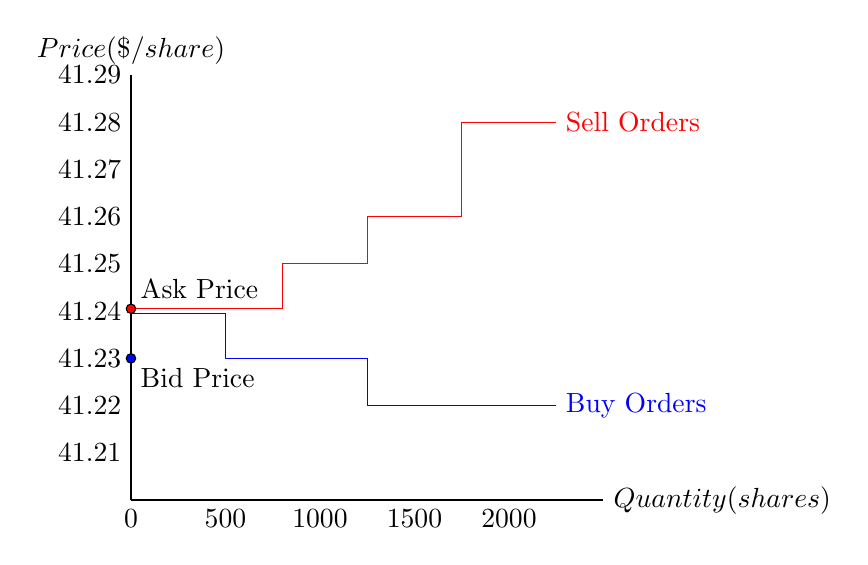
\begin{tikzpicture}[scale=.6]
        \draw[thick,-] (0,0) -- (0,9) node[above]{$Price (\$/share)$};
        \draw[thick,-] (0,0)--(10,0) node[right]{$Quantity (shares)$};
        \node[left] at (0,1) {$41.21$};
        \node[left] at (0,2) {$41.22$};
        \node[left] at (0,3) {$41.23$};
        \node[left] at (0,4) {$41.24$};
        \node[left] at (0,5) {$41.25$};
        \node[left] at (0,6) {$41.26$};
        \node[left] at (0,7) {$41.27$};
        \node[left] at (0,8) {$41.28$};
        \node[left] at (0,9) {$41.29$};
        \node[below] at (2,0) {$500$};
        \node[below] at (4,0) {$1000$};
        \node[below] at (6,0) {$1500$};
        \node[below] at (8,0) {$2000$};
        \node[below] at (0,0) {$0$};
        \draw[blue,solid] (0,3.95) -- (2,3.95) -- (2,3) -- (5,3) -- (5,2) -- (9,2) node[right]{Buy Orders} ;
        \draw[red,solid] (0,4.05) -- (3.2,4.05) -- (3.2,5) -- (5,5) -- (5,6) -- (7,6) -- (7,8) -- (9,8) node[right]{Sell Orders};
        \node[above right] at (0,4.05) {Ask Price};
        \draw[fill=red] (0,4.05) circle [radius=.1];
        \node[below right] at (0,3) {Bid Price};
        \draw[fill=blue] (0,3) circle [radius=.1];
        \end{tikzpicture}
        \caption{Standard Limit Order Book}
    \end{figure}
\end{frame}

\begin{frame}{Market Format 1: The Continuous Double Auction (CDA)}
    \begin{itemize}
        \item Since market supply and demand are discontinuous step functions of price, there is \textbf{no guarantee of a single point of intersection}: there can be excess of demand (supply), and often there is. 
        \item Hence, \textbf{an allocation rule} to determine $\alpha(t_0, t)$ is needed (time priority, or pro-rata)
        \item Often, orders are \textbf{prioritized} based on \textbf{the time they arrive}, so high speed is rewarded
        \item If an agent can \textbf{react to a relevant signal} (even if public) \textbf{faster} than other traders, she can \textbf{pick off stale orders} from other traders and reverse position after the information has spread in the market
        \item To avoid adverse price pressure, traders will want to \textbf{shred} large orders.
    \end{itemize}
\end{frame}

\begin{frame}{Market Format 2: The FLOW}
    \begin{itemize}
        \item Continuous scaled limit orders have \textbf{five parameters}: $\rightarrow$ ``\underline{Buy/Sell} up to a cumulative total of  \underline{$Q_{max}$} (shares) at maximum rate \underline{$U_{max}$} (shares per hour) at prices between \underline{$P_{L}$} and \underline{$P_{H}$} (dollars per share)."
        \item Consider a buy order, The buying rate or flow demand $U(p(t))$ is given by:
            \begin{align}
                U{(p(t))}=
                \begin{cases}
                    U_{max} & \text{ if } p{(t)} < P_{L} \\
                    (\frac{P_{H}-p(t)}{P_{H}-P_{L}})U_{max} & \text{ if } P_L \leq p{(t)} \leq P_H \\
                    0  & \text{ if } p{(t)} > P_{H} \\
                \end{cases}
            \end{align}
        where $p(t)$ is the clearing price at time $t$.
        \item Similarly, the flow supply $U(p(t))$ is also a function of $p(t)$
    \end{itemize}
\end{frame}

\begin{frame}{Market Format 2: FLOW - Example - Individual}
    \begin{figure}
        \centering
        
\includegraphics[width=\textwidth]{figures/flow.png}
        \caption{Continuous Scaled Limit Orders}
        \label{fig:flow}
    \end{figure}
\end{frame}

\begin{frame}{Market Format 2: FLOW - Example - Market}
    \begin{figure}[H]
        \centering
        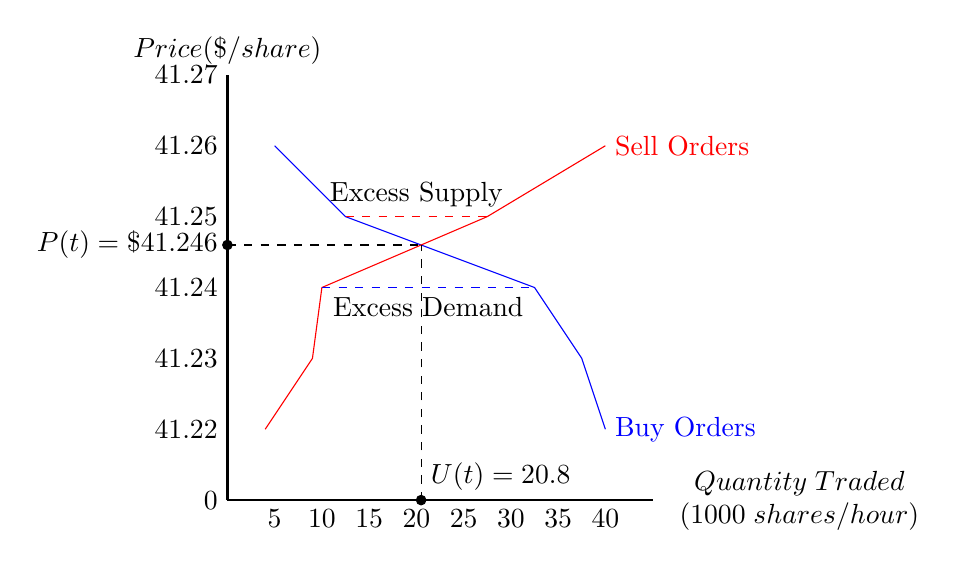
\begin{tikzpicture}[scale=0.6]
            \draw[thick,-] (0,0) -- (0,9) node[above]{$Price (\$/share)$};
            \draw[thick,-] (0,0)--(9,0) node[right]{\begin{tabular}{c}
                 $Quantity \; Traded$ \\
                 $(1000 \; shares/hour)$
            \end{tabular}};
            \node[left] at (0,1.5) {$41.22$};
            \node[left] at (0,3.0) {$41.23$};
            \node[left] at (0,4.5) {$41.24$};
            \node[left] at (0,6.0) {$41.25$};
            \node[left] at (0,7.5) {$41.26$};
            \node[left] at (0,9.0) {$41.27$};
            \node[below] at (1,0) {$5$};
            \node[below] at (2,0) {$10$};
            \node[below] at (3,0) {$15$};
            \node[below] at (4,0) {$20$};
            \node[below] at (5,0) {$25$};
            \node[below] at (6,0) {$30$};
            \node[below] at (7,0) {$35$};
            \node[below] at (8,0) {$40$};
            \node[left] at (0,0) {$0$};
            \draw[blue,solid] (1,7.5) -- (2.5,6.0) -- (6.5,4.5) -- (7.5,3) -- (8,1.5) node[right]{Buy Orders} ;
            \draw[red,solid] (0.8,1.5) -- (1.8,3) -- (2,4.5) -- (5.5,6) -- (8,7.5) node[right]{Sell Orders};
            \draw[red,dashed] (2.5,6.0) -- (5.5,6.0);
            \draw[blue,dashed] (2,4.5) -- (6.5,4.5);
            \node[black,above] at (4,6.0) {Excess Supply};
            \node[black,below] at (4.25,4.5) {Excess Demand};
            \draw[dashed] (4.1,0) -- (4.1,5.4);
            \draw[dashed] (0,5.4) -- (4.1,5.4);
            \node[above right] at (4.1,0) {$U(t)=20.8$};
            \draw[fill] (4.1,0) circle [radius=.1];
            \node[left] at (0,5.4) {$P(t)=\$41.246$};
            \draw[fill] (0,5.4) circle [radius=.1];
        \end{tikzpicture}
        \caption{Continuous Scaled Limit Order Book}
    \end{figure}
\end{frame}

\begin{frame}{Market Format 2: FLOW}
    \begin{itemize}
        \item Both the downward sloping demand schedule and upward sloping supply schedule are \textbf{piece-wise linear} functions of price $\rightarrow$ \textbf{unique} price and rate of shares per hour
        \item All continuous scaled limit orders ares treated \textbf{symmetrically} and executed \textbf{simultaneously} at the market clearing price
        \item \textbf{Opportunities} to do order \textbf{shredding} are now \textbf{distributed equally} across agents, as now instructions to shred are ``moved into the exchange"
        \item Consequently, now the \textbf{fastest trader} or the ones that can send massive number of messages to update orders are not rewarded
    \end{itemize}
\end{frame}

\section{Lab Procedures}

\begin{frame}{Experiment Design: Main Elements}
    \begin{itemize}
        \item Groups of 8 traders will participate in an asset market for 22 trading periods, each lasting two minutes (2 practice + 20 payment)
        \item \textbf{Incentives to trade}: In each trading period, the computer provides a buy or sell contract committing to buy or sell up to $x$ shares at some point during the trading period (e.g., Computer will buy up to 300 shares from you at price 13 ECUs at second 115)
        \item Contracts are private information
        \item Subjects' inventories are restricted to be $[-Q_{contract}, 0]$ for those with a sell contract or $[0, Q_{contract}]$ for those with a buy contract
        \item \textbf{Choice Space}: Subjects can submit or update buy and/or sell orders
        \item \textbf{Treatments}: \{CDA, FLOW\} (between-group)
        \item Three sets of contracts varied across 5 blocks of 4 periods each. 
    \end{itemize}
\end{frame}

\begin{frame}{Experiment Design: Contracts}
    \begin{figure}[H]
    \centering
    \begin{subfigure}{.33\linewidth}
        \centering
        \includegraphics[scale=0.12]{production/contract/production_1.png}
        \caption{Contract Set 1 (T1 - T4 \& T17 - T20)}
    \end{subfigure}%
    \begin{subfigure}{.33\linewidth}
        \centering
        \includegraphics[scale=0.12]{production/contract/production_2.png} 
        \caption{Contract Set 2 (T5 - T8 \& T13 - T16)}
    \end{subfigure}%
    \begin{subfigure}{.33\linewidth}
        \centering
        \includegraphics[scale=0.12]{production/contract/production_3.png}
        \caption{Contract Set 3 (T9 - T12)}
    \end{subfigure}
    \caption{Contract Design}
\end{figure}
\end{frame}

\begin{frame}{Experiment Design: Interface - FLOW}
    \begin{figure}[H]
        \centering
        
\includegraphics[width=\textwidth]{figures/flow_ui.png}
        \caption{FLOW UI}
        \label{fig:flow_ui}
    \end{figure}
\end{frame}

\begin{frame}{Experiment Design: Interface - FLOW Animation}
  \animategraphics[loop,controls,width=\linewidth]{10}{figures/flow_animation/flow_animation-}{0}{419}
\end{frame}

\begin{frame}{Experiment Design: Interface - CDA}
    \begin{figure}[H]
        \centering
        
\includegraphics[width=\textwidth]{figures/cda_ui.png}
        \caption{CDA UI}
        \label{fig:cda_ui}
    \end{figure}
\end{frame}

\begin{frame}{Experiment Design: Interface - CDA Animation}
  \animategraphics[loop,controls,width=\linewidth]{10}{figures/cda_animation/cda_animation-}{0}{252}
\end{frame}




\begin{frame}{Experiment Design: Procedures}
    \begin{itemize}
        \item We paid the cumulative profits of all 20 payment periods
        \item Exchange rate is 1000 ECUs = 1 USD and show-up fee is 7 USD
        \item Experiment software was designed and developed at UCSC's LEEPS Laboratory
        \item Experiment sessions were conducted in person at LEEPS Laboratory
        \item So far have 5 FLOW and 5 CDA sessions
    \end{itemize}
\end{frame}

\section{Results}

\begin{frame}{Results: Clearing Prices}
    \begin{figure}[H]
        \centering
        \begin{subfigure}[b]{\textwidth}
            \centering
            
\includegraphics[width=\linewidth]{figures/groups_flow_price.png}
            \caption{FLOW}
            \label{price_flow}
        \end{subfigure}
        \begin{subfigure}[b]{\textwidth}
            \centering
            \includegraphics[width=\linewidth]{figures/groups_cda_price_scatter.png}
            \caption{CDA}
            \label{price_cda}
        \end{subfigure}
        \caption{Clearing Prices}
    \end{figure}
    \vspace{-15pt}
    \scriptsize{The vertical dotted lines are period breaks. The first 10 seconds from each trading period are left out. The lighter colors represent individual groups.} 
\end{frame}

\begin{frame}{Results: Total Traded Volume}
    \begin{figure}[H]
        \centering
        \begin{subfigure}[b]{\textwidth}
            \centering
            
\includegraphics[width=\textwidth]{figures/groups_flow_cumsum.png}
            \caption{FLOW}
            \label{quantity_flow}
        \end{subfigure}
        \begin{subfigure}[b]{\textwidth}
            \centering
            
\includegraphics[width=\textwidth]{figures/groups_cda_cumsum.png}
            \caption{CDA}
            \label{quantity_cda}
        \end{subfigure}
        \caption{Total Traded Volume}
    \end{figure}
    \vspace{-15pt}
    \scriptsize{The first 10 seconds from each trading period are left out. The lighter colors represent individual groups.}
\end{frame}

\begin{frame}{Results: Realized Surplus}
    \begin{figure}[H]
        \centering
        \begin{subfigure}[b]{\textwidth}
            \centering
            
\includegraphics[width=.8\linewidth]{figures/groups_flow_surplus.png}
            \caption{FLOW}
            \label{surplus_flow}
        \end{subfigure}
        \begin{subfigure}[b]{\textwidth}
            \centering
            
\includegraphics[width=.8\linewidth]{figures/groups_cda_surplus.png}
            \caption{CDA}
            \label{surplus_cda}
        \end{subfigure}
        \caption{Realized Surplus}
    \end{figure}
\end{frame}

\begin{frame}{Results: Filled Contracts}
    \begin{figure}[H]
        \centering
        \begin{subfigure}[b]{\textwidth}
            \centering
            
\includegraphics[width=.8\linewidth]{figures/groups_flow_contract.png}
            \caption{FLOW}
            \label{contract_flow}
        \end{subfigure}
        \begin{subfigure}[b]{\textwidth}
            \centering
            
\includegraphics[width=.8\linewidth]{figures/groups_cda_contract.png}
            \caption{CDA}
            \label{contract_cda}
        \end{subfigure}
        \caption{Filled Contract}
    \end{figure}
\end{frame}

\begin{frame}{Results: Profits}
    \begin{figure}[H]
        \centering
        \begin{subfigure}[b]{\textwidth}
            \centering
            
\includegraphics[width=.8\linewidth]{figures/groups_flow_projected_profit_by_direction.png}
            \caption{FLOW}
            \label{profit_flow}
        \end{subfigure}
        \begin{subfigure}[b]{\textwidth}
            \centering
            
\includegraphics[width=.8\linewidth]{figures/groups_cda_projected_profit_by_direction.png}
            \caption{CDA}
            \label{profit_cda}
        \end{subfigure}
        \caption{Profits}
    \end{figure}
\end{frame}

\begin{frame}{Results: Summary Statistics}
    \begin{table}[H]
        \footnotesize
        \centering
        \resizebox{\textwidth}{!}{
        \begin{threeparttable}
        \centering
            \begin{spacing}{1.25}
            \begin{tabular}{lcccccc}
                \hline 
                \hline
                ~                                 & \multicolumn{2}{c}{T1 - T20}  & \multicolumn{2}{c}{T11 - T20} & \multicolumn{2}{c}{T1 - T10}\\
                ~                                 & FLOW          & CDA           & FLOW           & CDA        & FLOW       & CDA     \\
                \hline
                \hline 
                 Average Price                    & 9.36          & 8.57          & 9.26           & 8.27       & 9.44       & 8.81    \\
                                                  & (1.37)        & (1.37)        & (0.99)         & (1.28)     & (1.89)     & (1.98)  \\
                 Clearing Rate (shares/second)    & 9.35          & ~             & 9.77           & ~          & 8.98       & ~       \\
                                                  & (0.34)        & ~             & (0.17)         & ~          & (0.52)     & ~       \\
                 Quantity Traded per Match        & ~             & 74            & ~              & 68         & ~          & 80      \\
                                                  & ~             & (7.58)        & ~              & (9.29)     & ~          & (9.36)  \\
                 $\mid Price - P_{CE} \mid$       & 2.25          & 2.15          & 2.05           & 2.06       & 2.45       & 2.25    \\
                 Std($P_{t} - P_{t - 1}$)         & 1.37          & 2.88          & 1.34           & 2.76       & 1.4        & 3.02    \\
                 \#($P_{t} - P_{t - 1}$)          & 2194          & 736           & 1137           & 384        & 1057       & 352     \\
                 Total Traded Volume (shares/period) & 959           & 1138          & 1046           & 1179       & 872        & 1097    \\
                 Number of Orders     & 27            & 48            & 26             & 50         & 29       & 47      \\
                 Avg. Order Size (shares/period)                 & 35.9          & 20.8          & 40.2            & 19.9       & 31.6       & 21.7   \\
                \hline
                \hline
            \end{tabular}
            \end{spacing}
            \vspace{.5em}
            \begin{tablenotes}\noindent\justifying\scriptsize Standard deviations are in parentheses. All values are averages across the five groups that participated in each market. Prices, rates and quantities ignore values of zero. ($P_{t} - P_{t - 1}$) accounts for non-zero changes only. \end{tablenotes}
        \end{threeparttable}}
    \end{table}
\end{frame}

\begin{frame}{Results: Summary Statistics (Cont.)}
    \begin{table}[H]
        \footnotesize
        \centering
        \resizebox{\textwidth}{!}{
        \begin{threeparttable}
        \centering
            \begin{spacing}{1.25}
            \begin{tabular}{lcccccc}
                \hline 
                \hline
                ~                                 & \multicolumn{2}{c}{T1 - T20}  & \multicolumn{2}{c}{T11 - T20} & \multicolumn{2}{c}{T1 - T10} \\
                ~                                 & FLOW          & CDA           & FLOW           & CDA        & FLOW       & CDA          \\
                \hline
                \hline 
                 Realized Surplus (\%)            & 81.1          & 85.7          & 84.8           & 89.9       & 77.31      & 79.76        \\
                 Market Vol./Contract Vol. (\%)   & 72.1          & 79.6          & 78.9           & 83.5       & 65.39      & 75.82        \\
                 Profits (ECUs)                   & 1184.4        & 1222.8        & 1249.2         & 1287.6     & 1119.62    & 1157.94      \\
                                                  & (1106.0)      & (1127.6)      & (1126.9)       & (1161.4)   & (1082.3)   & (1090.3)     \\
                 \hspace{3mm}10-th percentile     & 0.6           & 0             & 1.8            & 0          & 0          & 0            \\
                 \hspace{3mm}50-th percentile     & 901.8         & 1001.5        & 962.5          & 1045.5     & 852.8      & 983          \\
                 \hspace{3mm}90-th percentile     & 2890.1        & 2800          & 2995.6         & 2944.2     & 2844.1     & 2682         \\
                 \hspace{3mm}Sellers              & 1053.29       & 890.66        & 1067.32        & 845.45     & 1039.26    & 935.88       \\
                                                  & (1035.92)     & (936.29)      & (1080.13)      & (871.15)   & (992.25)   & (997.33)     \\
                 \hspace{3mm}Buyers               & 1315.52       & 1554.84       & 1431.05        & 1729.69    & 1199.98    & 1379.99      \\
                                                  & (1158.52)     & (1203.44)     & (1145.92)      & (1246.12)  & (1162.37)  & (1135.60)    \\
                \hline
                \hline
            \end{tabular}
            \end{spacing}
        \vspace{.5em}
        \caption{Summary statistics for experimental data}
        \begin{tablenotes}\noindent\justifying\scriptsize Standard deviations are in parentheses. All values are averages across the five groups that participated in each market. Prices, rates and quantities ignore values of zero. \textit{Realized Surplus} is the proportion of the competitive equilibrium surplus that was obtained. \textit{Market Vol./Contract Vol.} is the proportion of the contract (infra-marginal) that was filled. \end{tablenotes}
        \end{threeparttable}}
    \end{table}
\end{frame}

\section{Conclusions}
\begin{frame}{Conclusions (Preliminary)}
    \begin{itemize}
    %\item No evidence of higher information efficiency 
    \item Price deviation is similar across the two formats.
    \item Price volatility is much lower in FLOW than in CDA. 
    \item Evidence of learning over time in FLOW, not so much in CDA. 
    \item After learning, FLOW does not show better price convergence, but do show some improvement, coming for higher rates of trading.
    \item Profit inequality more obvious in CDA than in FLOW. We plan to whether FLOW has leveling effects on profits. 
    \item Elements to be incorporated in experiment: heterogeneous messaging costs, costly reduction of latency, direct format competition. Other elements?
    \item Feedback is much appreciated.
    \end{itemize} 
\end{frame}



\end{document}